\section*{Abstract}

Zum einen können Lernen in unterschiedliche Typen unterteilt werden. Eine solche Unterteilung kann sowohl in Sozialformen wie es bei Schrader passiert ist, als auch in kompetenzbezogen wie es bei Zech der Fall ist vorgenommen werden. Zum anderen können Aufgaben unterschieden werden welchen Grad an Nützlichkeit ihre beigelegten Bilder haben. Diese Bilder können entweder nur dekorativen Nutzen haben, oder auch essenziell für das Lösen der Aufgabe sein und zusätzlich eine Anschauung vermitteln. In vorliegender Studie wurden 39 Studenten der TU München in einer Eyetrackingstudie zu den Fragestellungen untersucht: Lassen sich die Studenten in Lerntypen anhand ihrer Augenbewegungen einteilen? Wie wirkt sich der Lerntyp auf die Leistungsfähigkeit der Probanden aus? Und gibt es Lerntypen, die mit bestimmten beigelegten Bildern besser oder schlechter Umgehen können?  
Um diese Fragen zu Beantworten wurde den Studenten am Anfang ein heuristisches Lösungsbeispiel für einen mathematischen Zusammenhang gezeigt. Die Blickbewegungen der Studenten auf diesem Lösungsbeispiel legt die Lerntypunterteilung der Probanden fest. Im weiteren Teil wurden mathematische Aufgaben mit dekorativen und essenziellen Bildern gestellt, welche die Probanden bearbeitet haben. Eine Unterteilung der Lerntypen war in der mehrheit der Probanden möglich, jedoch die Unteschiede ihrer Leistungsfähigkeit nicht signifikannt. Bei der Verwendung unterschiedlicher Bildtypen, wurden aufgaben mit essenziellen Bildern etwas besser bearbeitet, wie Aufgaben mit nur dekorativen Bildern. Bei der Auswertung, wie die unterschiedlichen Lerntypen mit den beigefügten Bildern umgegangen sind war, dass Lernende, die im ersten Teil der Studie sehr viel auf Bilder geschaut haben, im zweiten Teil mit essenziellen Bildern nicht gut umgehen konnten.


\tableofcontents % Inhaltsverzeichnis

\chapter{Einleitung}

In der Ausbildung von Schülern, Schülerinnen (SuS) und Studenten ist es wichtig, dass die Lernenden
einen Weg finden sich Lernstoff anzueignen und diesen anwenden zu können. Lerntypen können in Auditiver-,
Visueller-, Motorischer-, und Kommunikativenlerntyp unterschieden werden.Wobei der Auditive gut über das Zuhören
lernt, der Visuelle über Veranschaulichungen lernt, der Motorische sich mit Bewegungenen Stoff aneignen kann und 
der Kommunikative den Lerngegenstand am besten aufnimmt, wenn er sich über ihn mit anderen spricht.  Somit sind diese Typen sehr unterschiedlich in ihrer Verwendung von Verarbeitungskanälen (Sinnesorganen).
Jeder dieser Typen Schaffst es am effektivsten auf verschiedene Art und Weiße sich neuen Stoff anzueignen.
Um dies zu gewährleisten, wird bereits im Lehrplanplus der Grundschule in Bayern festgehalten:
Es ist " Aufgabe aller Bildungsorte, in allen Lebensphasen und -bereichen individuelles (fett)
 Lernen anzuregen und so zu unterstützen, dass es lebenslang selbstverständlich wird."
 %https://www.lehrplanplus.bayern.de/leitlinien/grundschule
Hierbei entwickeln sich im Laufe der Schulbahn eigene Strategien, um komplexe Sachverhalte,
wie zum Beispiel mathematische Beweisse, zu erlernen. 
Im Umgang des Lernens aus Texten erscheint
es sinnvoll eine andere Lerntypunterteilung anzustreben, da Bilder oder Worte vorerst gelesen oder 
betrachtet werden müssen bevor sie verarbeitet werden können. Somit muss auch ein Auditiver- oder ein Kommunikativerlerntyp vorerst den Text lesen, um den Inhalt für sich zugreifbar zu machen. 

So wie sich die Lernenen in ihren Typen unterscheiden, sind die Hilfestellungen bei Aufgaben auch ganz unterschiedlich. Eine Aufgabenstellung kann nicht nur in ihrer kognitiven Prozessdimension (cognitive process Dimension), oder ihrer Wissensdimension(Knowledge Dimension), sondern auch in der Art der Unterstützung eingeteilt werden. Im mathematischen Konzext sind diese Unterstützungen meist Beispielrechungen oder Graphiken. Graphiken können laut (Zitation) in unterschiedliche Kathegorien eingeteilt werden, welche für die Bearbeitung der Aufgabestellung unteschiedlich hilfreich ist.% anderson und Krakwohl 2001

In vorliegender Studie soll sich auf die visuelle Wahrnehmung zurückgezogen werden und die Effektivität von unterschiedlichen Lerntypen im lösen von unterschiedlichen mathematischen Aufgabestellungen untersucht werden. 
\chapter{Theoretischer Hintergrund}

\section{Lerntypeneinteilung nach Gagné}

Gagné unterteilt seine Formen des Lernens hierarchisch, somit setzt meist die nachfolgende Lernart die vorhergehenden Lernarten voraus. Generell wird in zwei Teile unterteilt: 
\begin{itemize}
\item (A) Grundformen der Lernens: Assoziationen und Ketten 
    \begin{itemize}
        \item (A.1) Signallernen
        \item (A.2) Reiz-Reaktions-Lernen
        \item (A.3) Kettenbildung
        \item (A.4) Sprachliche Assoziation
    \end{itemize}
\item (B) Intellektuelle Fähigkeiten
    \begin{itemize}
        \item (B.1) Diskriminationslernen
        \item (B.2) Begriffslernen
        \item (B.3) Regellernen 
        \item (B.4) Problemlösen
    \end{itemize}
\end{itemize}

\subsection[]{(A.1) Signallernen (Pawlos "klassische" Konditionierungslehre)}

Man versucht mit einem Reiz eine dadurch bedingte Reaktion hervorzurufen. Eines der bekanntesten pädagogischen Phänomene hierfür ist der "Pawlowsche Hund". Hierbei wird immer bevor ein Hund Futter bekommt eine Glocke geschlagen. Nach vielen Druchgängen wird nur noch die Glocke geschlagen, was eine den Speichelfluss des Hundes anreizt, ohne das er Futter bekommt. Somit können einfache Reize ( z.B Ton) bestimmte Reaktionen (z.B Speichelfluss), welche nicht reflexartig angeboren sind, sondern an trainiert wurden, hervorrufen. %\cite Pawlos Konditionierungslehre

\subsection[]{(A.2) Reiz-Reaktions-Lernen (Trial and Error Prinzip, Lernen durch Verstärkung)}

Der Lernende versucht etwas so lang auf verschiedene Art und Weißen, bis es klappt und merkt sich anschließend wie man es gemacht hat. 
Beispiel: Jemand ist sich bei der letzten Nummer seines Fahrradschlosses unsicher. Er versucht deswegen einfach alle Möglichkeiten von 0 - 9 und merkt sich bei welcher Zahl das Schloss aufgegangen ist. Hierbei erfährt der Lernende eine Verstärkung, weil er danach mehr kann als davor ( in unserem Beispiel :Schloss öffnen) und dies nur durch einfaches Ausprobieren geschafft hat.

\subsection[]{(A.3) Kettenbildung (Lernen von Abläufen)}

In diesem Fall werden längere Reiz-Reaktions-Ketten gebildet. Hierbei sind alle Formen von Algorithmen oder Verfahren gemeint. Beispiele: Kochen, Telefonieren, oder auch Klammern im Mathematikunterricht auflösen. Diese Ketten können meist verstanden und durchgeführt werden, ohne einen tieferen Sinn des einzelnen Verfahrens verstanden zu haben. In der Schule kann diese Lernart zu Problemen führen, da die SuS (Schüler und Schülerinnen) kein Verständnis für die Zusammenhänge haben müssen, sondern nur ihre Algorithmen durchgehen können. Dies kann in Aufgaben mit höherem Abstraktionsgrad zu Problemen führen, wenn ihr Schema nicht mehr ohne weiteres anwendbar ist.

\subsection[]{(A.4) Sprachliche Assoziation (verbales auswendig Lernen)}

Hierbei werden bestimmte Definitionen, Gedichte oder Ähnliches einfach so lange wiederholt, bis sie auswendig vom Lernenden vorgetragen werden können. Hierbei findet somit eine Verkettung oder auch Assoziation von einfachen Objekten, in unserem Fall Wörtern, statt. Hierbei ist werden ebenso, wie in den anderen Grundformen, lediglich die Verknüpfungen der Wörter geschaffen und kein Verständnis dabei erzeugt. 

\subsection[]{(B.1) Diskriminationslernen (Unterscheidungslernen)}

In diesem Fall soll der Lernende verschiedene Gegenstände und Merkmale als verschieden auffassen können. Beispiele: Ein bestimmtes Passwort passt nur zu einem bestimmten Account, oder: nicht jedes Fahrrad schaut gleich aus, es gibt Rennräder, Stadträder, Lastenräder uvm.  . Somit soll der Lernende in besseres Verständnis für Begriffe entwickeln, indem er lernt diese zu differenzieren.

\begin{figure}[!ht]
\noindent\hspace{0.5mm}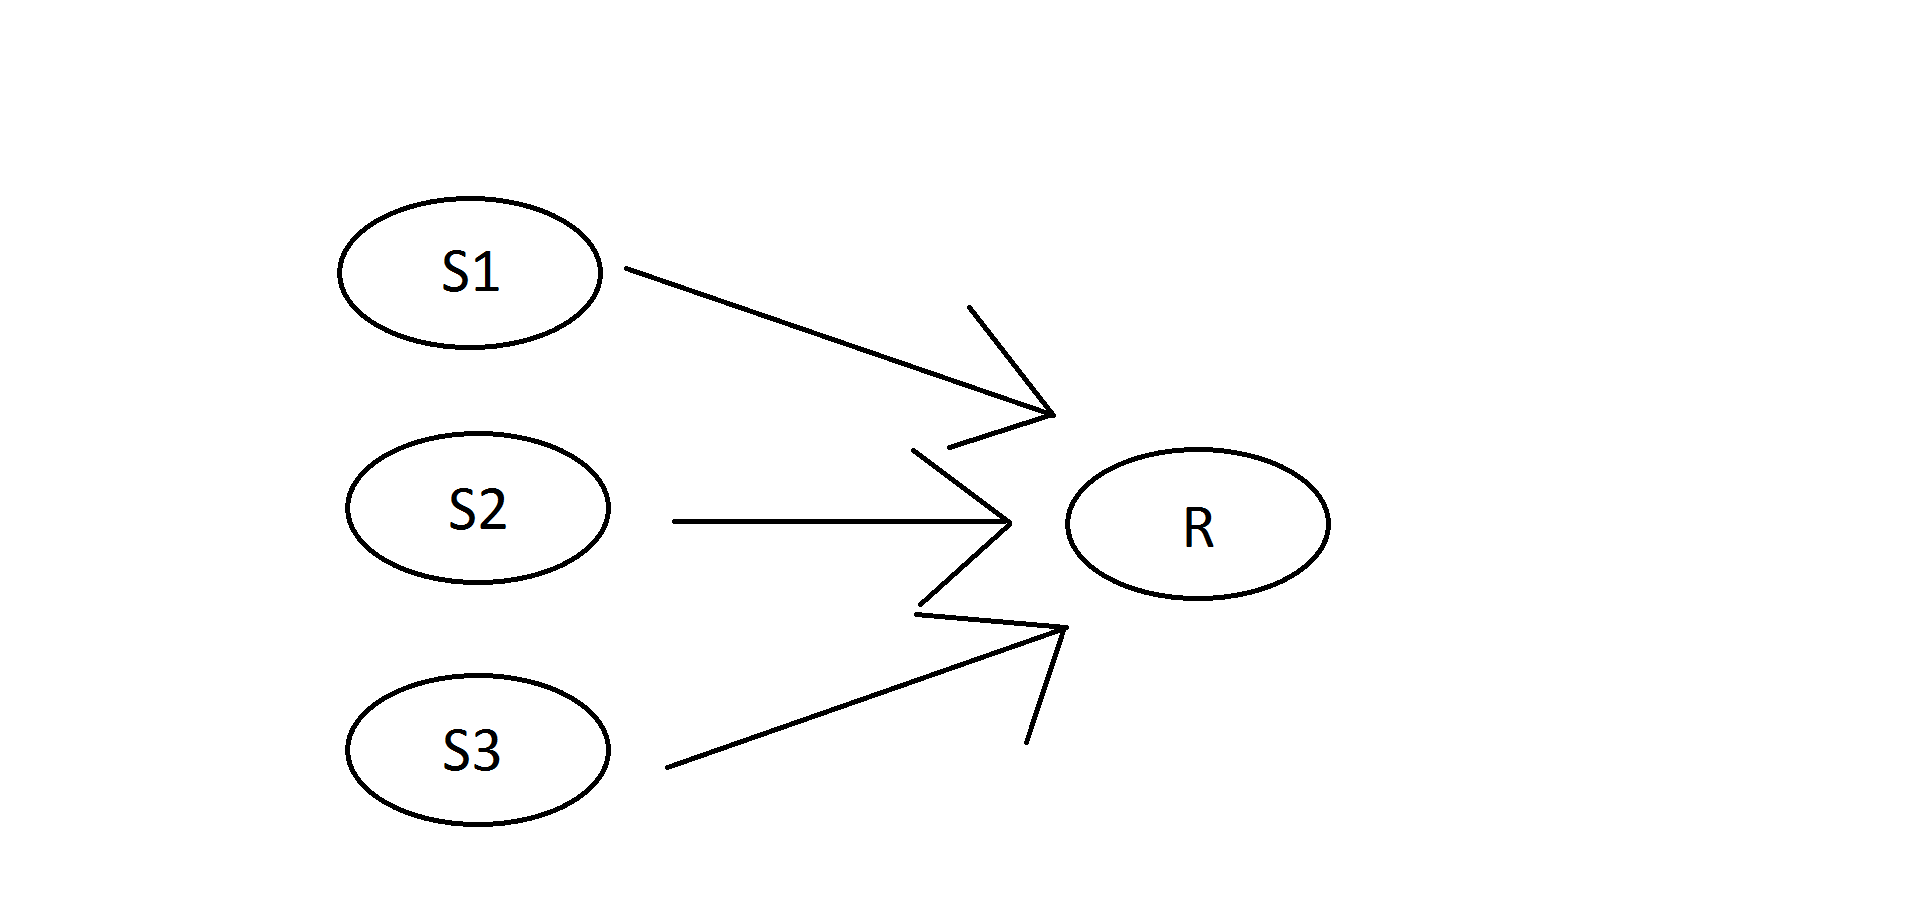
\includegraphics[width=12cm]{./Ressourcen/Diskrimination.png}
\caption{Diskriminationsleren, Zech}
\end{figure}

\subsection[]{(B.2) Begriffslernen (Gemeinsamkeiten finden)}

Bei diesem Typ soll genau der andere Weg wie im Diskriminationslernen gegangen werden. Hierbei sollen unterschiedliche Objekte als gleich zusammengefasst werden können. 
Beispiele: ein Rechteck und ein Quadrat sind beides Vierecke, oder ein Audi Q7 und ein BMW 5er sind beides Autos. Somit können besser Verbindungen zwischen Lerngegenständen hergestellt werden und sich auf allgemeine Details zurückgezogen werden (z.B Winkelsumme Viereck sind 360 Grad, Auto hat einen Motor).

\begin{figure}[!ht]
\noindent\hspace{0.5mm}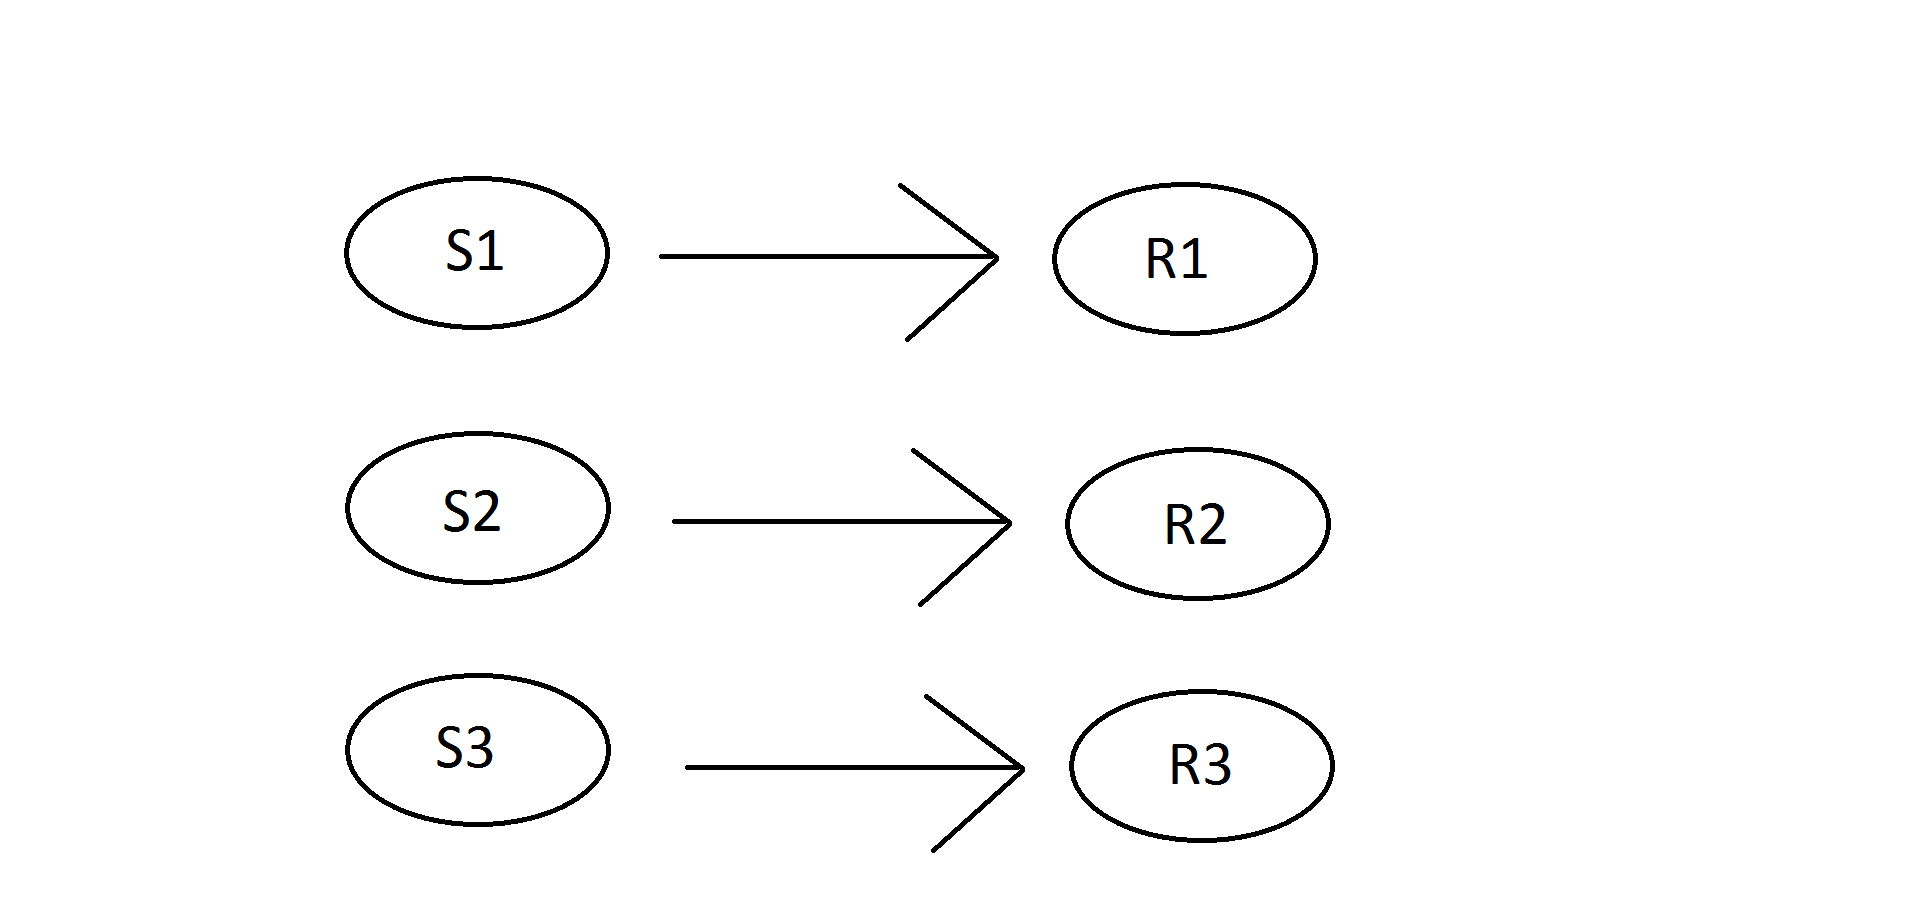
\includegraphics[width=12cm]{./Ressourcen/Begriffslernen.png}
\caption{Begriffslernen, Zech}
\end{figure}

\subsection[]{(B.3) Regellernen (Regeln auf Anwendungsbereiche lernen)}

Hierbei ist nicht nur das einfache auswendig lernen von Regeln oder der gleichen gemeint, sondern auch das damit verbundene Verständnis. Somit kann das Regellernen als im Kontext des Satzes von Pythagoras aufgefasst werden: Das zum einen die Formel $a^2$ + $b^2$ = $c^2$ im aktiven Wissen vorhanden ist, als auch die Anwendung und die Bedingungen der Formel verständlich sind.

\subsection[]{(B.4) Problemlösen (Aufgaben mit eigenen Überlegungen lösen)}

Dies ist der nächste Schritt von dem Regellernen, da hierbei Regeln verstanden sein müssen und diese kombiniert in einer Aufgabe angewendet werden können. Somit gehört in der gagnéschen Hierarchie der Problemlöser zur höchsten Ordnung, da seine Kompetenzen die Kompetenzen der vorhergehenden Typen beinhalten.

\section{Lerntypeneinteilung nach Zech}

Die Lerntypen von Gagné werden in der Einteilung nach Zech aufgegriffen, zusammengefasst und erweitert um neue Lerntypen zu definieren. Ebenso betrachtet er die Lerntypen hauptsächlich im Kontext der Mathematik und nicht mehr Allgemeinen. Zech unterteilt seine Lerntypen nicht mehr Hierarchisch wie zuvor passiert ist und gibt klare Lernbedienungen für den jeweiligen Lerntypen an. Es werden die folgenden 7 Typen betrachtet:

\subsection[]{Assoziatives Lernen}

In dieser Unterteilung sind die im kognitiven Bereich beschränkten Grundformen des Lernens (Teil A) nach Gagné zusammengefasst. Somit werden bei diesem Typ "kürzere oder längere Reiz-Reaktions-Verbindungen (Automatismen)" aufgebaut und diese hauptsächlich auswendig gelernt. Dies kann man im Mathematischen Sinne als das Anwenden von bekannten Regeln auf einfache Aufgabentypen verstanden werden. Ebenso bezieht sich dieser Typ über die Abstammung von den Grundformen (A) mehr auf textuelle Teile von Aufgaben, als auf bildliche Teile.
Die Lernbedingung dieses Types ist: häufige Wiederholung. 
Aus diesem Typ entsteht in der Unterteilung des Versuchaufbaus dieser Arbeit die Gruppierung "Textueller", welche sich dadurch auszeichnet das heuristische Beispiel sehr häufig wiederholt durchliest und sich somit, nach dem ersten durchlesen weiter auf den Text fokussiert. 


\subsection[]{Diskriminationslernen}

Er wird zu großen Teilen aus dem Typ von B.1 abgeleitet, wie der Name auch schon vermuten lässt. Hierbei wird aber nochmal verdeutlicht, dass das Diskriminationslernen als Voraussetzung zum Begriffslernen stehen muss, da erst Objekte unter einem Begriff zusammengefasst werden können, bevor sie als unterschiedlich erkannt werden können.
Lernbedingungen: Unterschiede hervorheben (zum Beispiel mit bunter Kreide), Kontiguität (Angrenzung, Berührung)%\cite"https://www.duden.de/rechtschreibung/Kontiguitaet".
Dieser Lerntyp ist in der gegebenen Studie schwer von den anderen Typen zu unterscheiden, da sich die Aufgabenstellung nicht explizit mit Diskrimination befasst, sondern mit dem lösen mathematischer Probleme. Somit wird dieser Lerntyp in der Studie nicht weiter behandelt.

\subsection[]{Lernen mathematischer Begriffe}

Dieser Typ baut sich auch auf dem Lerntyp B.2 Begriffslernen auf. Hierbei werden vorerst die Begriffe unterteilt in: Eigenschaftsbegriffe, Relationsbegriffe und zusammengesetzte Begriffe. Eigenschaftsbegriffe beschreiben Merkmale oder Eigenschaften eines Objektes. Relationsbegriffe beschreiben eine Relation zwischen verschiedenen Objekten, wie z.B A hat mehr Kanten wie B. Zusammengesetzte Begriffe werden aus einer Kombination von ursprünglichen Begriffen definiert z.B \textit{ eine Teilmenge des euklidischen Raums R n heißt kompakt, wenn sie abgeschlossen und beschränkt ist}. Diese Begriffe sollen durch die zusammenstezung mehrere bekannter Begriffe verstanden werden. Dieser Lerntyp auf B.3 Regellernen auf. Die Begriffe gehen durch Abstraktion aus der Erfahrungswelt hervor.
Lernbedingungen: relevante Merkmale hervorheben, mehrere Beispiele(irrelevante Merkmale variieren), Gegenbeispiele.
Leider sind die gegebenen Lernbedingungen an Hand einer Eyetracking-Studie, bei der nichts markiert werden kann, oder der Proband Beispiele und Gegenbeispiele anbringen kann, nicht auszuwerten. Aus diesem Grund wurde dieser Lerntyp ebenso in der Studie nicht weiter behandelt. 

\subsection[]{Lösen mathematischer Probleme}

Unter diesem Lerntyp wird ein verinnerlichen mathematischer Zusammenhänge verstanden. Hierbei wird das lernen von heuristischer Regeln vorausgesetzt. Es müssen zuerst bestimmte allgemeine Strategien (z.B Widerspruchsbeweis) aufgenommen werden, um anschließend eine Transferleistung zu vollbringen, wie es in Aufgaben mit hohem Abstraktionsgrad vorausgesetzt wird. 
Lernbedingungen: Problemlösefahigkeiten (analysieren, vergleichen, Beziehungen herstellen uvm), Fähigkeit, heuristische Regeln einzusetzen.
In Anlehnung an den Typ "Lösen mathematischer Probleme" wird in meiner Arbeit die Gruppierung "Problemlöser" definiert, welche sich sehr stark auf die Bilder fokussiert nachdem er den Text das erste mal durchgelesen hat.

\section{Lerntypeneinteilung nach Schrader}

Wie bereits angedeutet unterteilt Schrader seine Lerntypen eher in Sozialformen: der Theoretiker, der Anwendungsorientierte, der Musterschüler, der Gleichgültige und der Unsichere. Hierbei werden nicht mehr alle Typen aufgelistet, da viele sich in den Typen von Zech widerspiegeln und in der Studie nicht die Sozialformen berücksichtigt wurden. Somit wird nur auf den Typ "der Unsichere" eingegangen.

Der "Unsichere" sucht Ursachen bei sich und zweifelt an seinen Fähigkeiten. Das lernen aus Texten fällt diesem Typ schwer, da er wenig systematisch dabei vorgeht. Er lässt sich lieber etwas mehr Zeit und die gegebene Aufgabenstellung zu bearbeiten.
Lerncharakteristik: Da ihm das arbeiten mit Texten Schwierigkeiten bereitet, ist die Bearbeitungszeit länger als gewöhnlich und es werden sowohl im textuelle Bereiche als auch Bildbereiche häufiger betrachtet, als bei einem gewöhnlichen Probanden es der Fall wäre. 

\section{Mehrgewinn von Graphischen Darstellungen}

Laut einer Studie von (Mayer,2005), hat das Arbeitsgedächtniss zwei Kanäle zur Verarbeitung von Informationen. Einer der Kanäle verarbeitet Informationen von Wörtern und der andere von Bildern. Somit kann eine optimale Lernbedingung geschafft werden, indem sowohl verständlicher Text als auch passende (eingebundene) Bilder dem Lernenden zu Verfügung gestellt werden. Laut Matthias Böckmann und Stanislaw Schukajlow (2018) lassen sich Bilder in drei unterschiedliche Typen unterteilen:
    
    \begin{itemize}
        \item dekorative Bilder (Decorative pictures), welche keine echten Informationen über das gegeben Problem geben. Zum Beispiel eine Radfahrerin, wenn es in der Aufgabe über das Zurücklegen einer Strecke mit dem Rad geht.
        \item repräsentative Bilder (Representational pictures), welche Teile der gestellten Aufgabe veranschaulichen. Zum Beispiel ein Drachenviereck, wenn die Aufgabe gestellt ist: den Flächeninhalt eines Drachenvierecks zu bestimmen. 
        \item essenzielle Bilder (Essential pictures), welche Informationen geben die essenziell sind für die Bearbeitung der Aufgabe. Zum Beispiel bei der Berechnung einer Fläche, ein Graphik in der relevante längen von Seiten eingetragen sind.
    \end{itemize}

In ihrer Studie wurden 217 SuS aus der 9. Klasse in Gruppen eingeteilt. Bei dem Versuch wurden die SuS in drei Gruppen unterteilt, welche die selbe Aufgabenstellung bekommen haben, jedoch die Bildtypen sich unterschieden haben. In der Aufgabe wird von den SuS verlangt den Abstand von einer Person zu ihrem Lenkdrachen, mit hilfe des Satzes von Pythagoras, zu berechnen. Die Aufgabestellung sollte von den SuS nicht bearbeitet, sondern lediglich Fragen hierzu beantwortet werden. 
Die erste Gruppe hat eine Aufgabenstellung mit einem dekorativen Bild gestellt bekommen. Hierbei ist nur ein Bild eines Lenkdrachen gezeigt.
Die zweite Gruppe hat ein Bild erhalten in dem die beschriebene Situation bildlich dargestellt wurde (repräsentativ). Hingegen hat die dritte Gruppe das selbe Bild wie die zweite Gruppe erhalten, nur mit längenangaben im Bild (essenziell).
Es konnte gezeigt werden, dass dekorative Bilder den Probanden kaum eine Unterstützung in der Lösung der gestellten Aufgaben geben. Hingegen repräsentative einen positiven Effekt haben und essenzielle Bilder den besten Effekt haben.%cite

\chapter{Methodik}

\section{Eyetracking}

In dieser Studie wurde die Methode des Eyetrackings benutzt um die Blickbewegungen der Probanden auf dem Bildschirm fest zu halten. Im folgenden wird kurz die Einrichtung und die Funktionsweise eines Eyetracking Monitors beschrieben. 

Geräte, welche Blickbewegungen aufzeichnen können unterscheiden sich in zwei grundlegende Kathegorien:
    \begin{itemize}
        \item die eine Aufzeichnung über eine Brille erstellen
        \item die eine Kamera unterhalb des Bildschirms verwenden
    \end{itemize}


In diesem Versuchsaufbau wurde die 2. Variante gewählt. Hierbei ist es sehr wichtig, dass der Proband auf der richtigen Höhe sitzt und einen ungehinderten Blick (keine Brille) auf den Bildschirm hat. Ebenso wichtig ist, dass der Proband seinen Kopf gerade hält und nur die Augen bewegt, bei einer übermäßigen Bewegung des Kopfes werden die aufgezeichneten Daten verfälscht. Bevor mit der eigentlichen Studie begonnen werden kann, muss die Kamera kalibriert werden, hierfür soll der Versuchsteilnehmer einem Punkt am Bildschirm folgen um eine richtige Einstellung des Gerätes hervor zu rufen. 

Der Versuchsaufbau ist wie in der Abbildung beschrieben, dass der Proband (P) vor dem Bildschirm mit Kamera sitzt und der Versuchsleiter (V) auf der anderen Seite des Bildschirms. Die Kamera, welche die Blickbewegungen des Probanden aufzeichnet sitzt unter dem Anzeigebildschirm. Dieser Aufbau wurde gewählt, damit der Proband einfach ``weiter'' oder das Ergebnis einer Aufgabe sagen kann ohne den Blick vom Anzeigebildschirm zu lösen. Bei einer der Verwendung einer Tastatur, würde der Proband jedes mal wenn er auf sie schaut, die Kalibrierung des Eyetrackinggerätes verändert und somit die Daten verfälschen. 

\begin{figure}[!ht]
\noindent\hspace{0.5mm}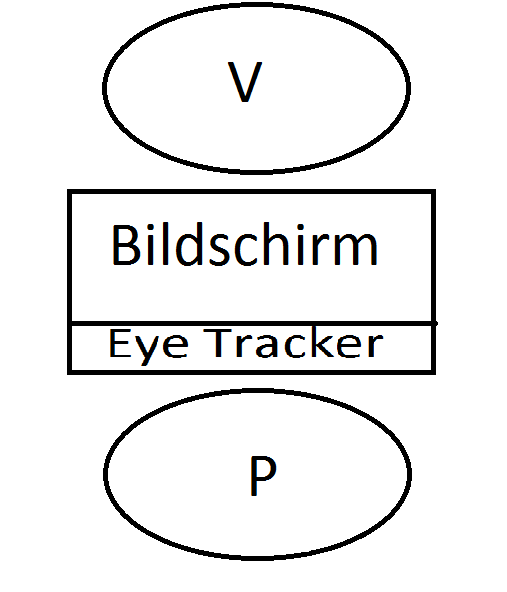
\includegraphics[width=8cm]{./Ressourcen/Versuchsaufbau.png}
\caption{Diskriminationsleren, Zech}
\end{figure}

\section{Begriffserklärung und Instrumentbeschreibung}
Um diese Studie nachzuvollziehen werden im folgenden Teil einige Begriffe erklärt und angegeben wie die Daten ausgewertet wurden. 

Beginnend mit dem Begriff Fixationen auf ein bestimmtes Objekt ist in dieser Studie ein messbares innehalten des Probanden auf einer Bestimmten Stelle des Bildschrims gemeint.``Diese Zeitdauer beträgt typischerweise 100 bis 200ms.'' %ftp://ftp.informatik.uni-stuttgart.de/pub/library/medoc.ustuttgart_fi/DIP-3183/DIP-3183.pdf

Somit sind die Fixationen bei einer Auswertung von Eyetrackinguntersuchungen immer in drei Teile unterteilt:
    \begin{itemize}
        \item Die Koordinaten der einzelnen Fixation, meist aufgeteilt in einen x und einen y Wert.(Horizontal, Vertikal)
        \item Die Dauer der jeweiligen Fixation
        \item Die zeitliche Reihenfolge der Fixation
    \end{itemize}

Durch AOIs (``Area of Interrest'') kann der für den Probanden sichtbare Bereich des Bildschirms in Abschnitte unterteilt werden, welche für die Auswertung relevant sind. In forliegender Studie wurden auf der ersten Seite AOIs über die Textabschnitte, sowie über die Graphiken legt um die Fixationen auf diesem Bereich feststellen zu können. Ebenso wurde in den letzten Bereich eine AOI gelegt um das Unterscheiden von dem ersten zum zweiten Druchgang zu ermitteln (mehr dazu im Teil eigene Einteilung).

Eine Heatmap ist eine Darstellung des Bildschirms, in der die Benutzerfixationen anhand von ihrer Häufigkeit und Dauer eingefärbt werden. Hierbei können Zonen, welche vom Benutzer intensiv Betrachtet werden schnell veranschaulicht werden.

Diese Daten wurden mit Hilfe des Eyetrackingapperates RED 500 festgehalten und konnten in unter Verwendung des Programms IViewx unterteilt werden. Somit konnte die Anzahl der Fixationen in einem Bereich ausgewertet werden. Diese Daten wurde verwendet um die Gruppeneinteilung im folgenden Verlauf der Arbeit vorzunehmen.

Nach der Einteilung der Gruppen wurden zum einen Varianzanalysen zu den gegebenene Forschungsfragen angestellt. Die Auswertung erfolgte über einen Einfaktorielle ANOVA um signifikante Unterschiede in den Gruppen oder unter den Bildern festellen zu können. Zum anderen wurden die Mittelwerte berechnet und verglichen. Diese Auswertungen sind im Teil Ergebnis festgehalten.

\section{Ablauf der Studie}

Auf der ersten Folie wurde den Versuchsteilnehmern ein teilbarkeits Beweiß von 3 oder 5 aufeinander folgender Zahlen anhand eines Heuristischem Lösungsbeispiels veranschaulicht. Hierbei wurde gezeigt, dass 3 aufeinanderfolgende Zahlen z.B 3,4,5 in der Summe, also in unserem Bespiel 12, wieder durch die Anzahl der aufeinander folgenden Zahlen Teilbar mit Ganzzahligem Ergbniss ist. Somit kann in unserem Beispiel die 12 durch 3 geteilt werden, ohne einen Rest zu haben.
Analog funktioniert es bei jeder ungeraden Anzahl an aufeinanderfolgender Natürlicher Zahlen. Die erste Folie unterteilt sich in Heuristiken, welche den algemeinen Lösungsweg des Beweißes aufzeigen sollen und in Inhalt, welcher von textueller und bildlicher Form sein kann. In bildlicher Form ist zum einen ein Anfangsbespiel, bei dem die Hypothese bei unterschiedlichen Zahlen überprüft wird, und zum anderen eine Möglichkeit, wie man durch Sortierung den Sachverhalt besser zu veranschaulichen. Im textueller Form wurden die Überlegungen festgehalten.

Darauf folgend wurden den Probanden 9 mathematische Aufgaben gestellt, welche sie mit Hilfe einer multiple choice Antwortmöglichkeit beantworten sollten. Ein Beispiel für eine Aufgabe ist:

\section*{Frage 1: HEIKE DIE RADFAHRERIN}

Auf einer Tour ist Heike 4 km in den ersten 10 Minuten gefahren und dann 2 km in den
nächsten 5 Minuten.


Welche der folgenden Aussagen ist richtig?

Antwortmöglichkeiten(fett):
    \begin{itemize}
        \item A(fett) Heikes Durchschnittsgeschwindigkeit war in den ersten 10 Minuten größer als in den nächsten 5
            Minuten.
        \item B(fett) Heikes Durchschnittsgeschwindigkeit war in den ersten 10 Minuten und in den nächsten 5
            Minuten die gleiche.
        \item C(fett) Heikes Durchschnittsgeschwindigkeit war in den ersten 10 Minuten niedriger als in den nächsten
            5 Minuten.
        \item D(fett) Es ist nicht möglich, anhand der Angaben etwas über Heikes Durchschnittsgeschwindigkeit zu
    \end{itemize}


\section{Eigene Gruppeneinteilung}

Aus den oben genannten Lerntypen wurden drei Gruppierungen gebildet: Typ 1 der Unsichere, Typ 2 der Problemlöser, Typ 3 der Textuelle. Die gegebenen 39 Probanden wurden in die vorliegenden Typen unterteilt nach folgender Tabelle. 22 der Versuchsteilnehmer konnten in jeweils eine der Gruppierungen unterteilt werden. Bei den restlichen 17 war dies leider nicht möglich. Das erstmalige lesen des Textes dauerte dauerte im Schnitt über alle Probanden 110,4 Sekunden. Diese Messung konnte festgestellt werden, indem am Ende des Textes Fixationen in einer AOI festgestellt wurden. Sobalt also ein Proband in dieses Feld geblickt, ist der erste Durchgang des Lesevorgangs beendet und der Zweite beginnt, welcher andauert, bis der Proband auf die nächste Folie wechselt. Diese Einteilung konnte anhand von Messungen der Zeit und der Reihenfolge der Fixationen belegt werden. 

Die Probanden wiesen in der Allgemeinheit noch folgenden Werte im Durchschnitt auf:
    \begin{itemize}
        \item Dauer des Zweiten Durchgangs: 72,6 Sekungen 
        \item Fixationen auf die Bildbereiche im zweiten Durchgang: 75,2
        \item Fixationen auf die Textbereiche im zweiten Durchgang: 71,1
    \end{itemize}

Die Probanden wurden auf die genannten Merkmale untersucht und in die passen den Gruppen anhand dieser Einteilung zugeordnet.
\section*{Einteilungsschema}

\begin{table}[!h]
\hspace{-5pt}
\begin{tabularx}{\textwidth + 5pt}{| @{\hspace{3pt}} M || @{\hspace{3pt}} M  | @{\hspace{3pt}} M  | @{\hspace{3pt}} M |}
\hline
\textbf{Ausprägungen} & \textbf{Typ Unsicher} & \textbf{Typ Problemlöser} & \textbf{Typ Textuell}\\
\hline
\hline
Dauer 1. Durchgang          & (+) & 0 & 0\\
\hline
Dauer 2. Durchgang          & ++ & 0 & (+)\\
\hline
Textfixationen 2. Durchgang & + & 0 & +\\
\hline
Bildfixationen 2. Durchgang & + & + & 0\\
\hline
\end{tabularx}
\caption{Ausprägungen}
\end{table}

\section{Eigene Aufgabe-Bildeinteilung}

In dieser Studie wurden die zugegebenen Bilder und Graphiken wie folgt unterteilt:

In ersten beiden Aufgabestellungen geht es um eine Radfahrerin, wobei lediglich ein Bild dieser Radfahrerin abgebildet ist. Dieses Bild trägt nicht zur Veranschaulichung oder Unterstützung der Versuchsperson bei und ist somit dekorativ. 


In der nächsten Aufgabenstellung ist ein Graph über die Geschwindigkeit eines Rennfahrers in Abhängigkeit vom Weg zu sehen. Dieser Graph muss verwendet werden, um die Aufgabenstellung zu bearbeiten und ist somit essenziell. 


In der darauf folgenden geschilderten Problematik sind 2 Graphiken, welche Teile eines Zufallsexperimentes darstellen verwendet. Hierbei müssen die Felder des Glücksrades und die Verteilung der Kugeln betrachtet werden um die Aufgabenstellung lösen zu können und somit sind die Graphiken auch essenziell.


Die nächsten beiden Aufgaben handeln vom Bergsteigen, hierbei ist lediglich ein Berg als Bild gegeben, welcher aber für die Bearbeitung der Aufgabe aber nicht nützlich ist, somit ist das Bild dekorativ. 


Im Anschluss wird noch eine Aufgabe im Themenbereich des Autofahrens gegeben. Dabei wurde wiederum ein Graph verwendet, der die Geschwindigkeit und die Zeit der Autfahrerin in Relation setzt. Diese Graphik ist wiederum essenziell für die Bearbeitung der Aufgabe. 


In den letzten beiden Aufgabestellungen wurde sowohl eine Tabelle, welche essenziell für die Bearbeitung ist, als auch ein einfaches Bild von einem Auto, welches eher dekorativen Charakter hat, verwendet. Da hierbei eine Mischung von Bildtypen verwendet wurde werden diese beiden Aufgaben in der weiteren Bearbeitung nicht weiter betrachtet. 

Somit kommen in dieser Bildunterteilung lediglich drei essenzielle und vier dekorative Bilder vor und keine representativen Bilder. Somit sollte der Unterschied zwischen hilfreichen und nicht hilfreichen Bildern besser sichtbar sein.

\section{Schwierigkeiten bei der Erfassung}

Bei der Erfassung der Punkte einer Aufgabe ist lediglich ein Punkt vergeben worden, wenn die Aufgabe richtig gelöst wurde und kein Punkt vergeben worden, wenn die Lösung nicht stimmt, somit werden keine Teilpunkte vergeben. Wenn ein Proband die Aufgabe zu Teilen richtig löst, anschliesend aber sich einen Denkfehler erlaubt bekommt er dennoch 0 Punkte auf die Aufgabe. Hierbei findet somit eine ergebnisorientierte- und keine lösungswegorientierte Auswertung der Aufgaben statt, welche die Fähigkeiten der Probanden schlechter abbildet als sie eigentlich wären.

Zusätzlich wurden Multiplechoice Antwortmöglichkeiten gegeben. Diese beiden Vorraussetzungen erzeugen eine unschärfe der Antwort des Probanden. Eine Verbesserung der Leistung des Probanden wird durch die vierfache Antwortmöglichkeit der Aufaben gegeben, da der Proband durch raten der Richtigen Lösung mit einer Warscheinlichkeit von 1/4 oder 25 Prozent richtig liegt. Dies hat zur Folge, dass die Fahigkeiten der Probanden besser abgebildet werden als sie eigentlich wären.  

Ebenso war es für die Probanden nicht möglich sich Aufgabenteile zu markieren, oder sich Notizen oder Rechnungen auf Papier nebenbei zu machen, dies hätte Kalibierungsprobleme des Eyetrackingautomaten hervorrufen können. Dies könnte man meinen, sollte sich auch negativ aus die Auswertung der Aufgaben auswirken, jedoch haben Schukajlow und Leiss (2011) gezeigt, dass ``(b)ezüglich der selbstberichteten Strategienutzung und der mathematischen Modellierungsleistungen der Lernenden konnten keine signifikanten Korrelationen festgestellt werden.'' Somit dieser Punkt nicht mit Sicherheit als ein Nachteil des Probanden gewertet werden. 

Die Einschränkungen der Ergebnissauswahl und der nur ergebnissorientierten Auswertungsansatz haben die Auswertung der Studie deutlich vereinfacht und wurden deswegen so gewählt. Zusätzlich könnten sich auch beide Effekte im besten Fall aufgehoben haben.  

\section{Forschungsfrage}
Texte werden von den Versuchsteilnehmern unterschiedlich bearbeitet, hierbei liegen unterschiedliche Teilbereiche in textueller oder in bildlicher Form im Fokus. Häuftig ist das lesen beim ersten Mal ein relativ linearer Vorgang, von links nach rechts und dann von oben nach unten gelesen. Nach dem ersten Durchgang unterscheiden Sich die Probanden und einzelne Teilbereiche des Textes werden einer weiteren Betrachtung unterzogen. Dies führt uns zu der Frage:
(1) Kann man die Probanden anhand ihrer Augenbewegungen in Gruppen unterteilen, (2) ob die Unterteilung Aufschlüsse die Leistungsfähigkeit innerhalb der Gruppe gibt?

Ein weitere Teil der Studie ist, das Ergebniss von Matthias Böckmann und Stanislaw Schukajlow (2018) in unserer Studie zu verifizieren (3), indem die unterteilten Aufgaben und die Gesamtpunktzahl der jeweiligen Aufgabe betrachtet wird. Somit wird untersucht ob ein direkter Zusammenhang zwischen der Lösung der Aufgabe und dem Typ des verwendeten Bildes besteht. Zuletzt wird noch untersucht, ob bestimmte Aufgabentypen für einzelne Probandengruppen positive oder auch negative Auwirkungen haben (4).

\chapter{Ergebniss}

Die in der Stuide getesteten Probanden waren Studenten der TU München und wiesen die folgenden Werte auf:

    \begin{itemize}
        \item 35,9 Prozent von ihnen waren weiblich 
        \item die Probanden kamen überweigend aus Bayern 66,7 Prozent
        \item das Druchschnittsalter lag bei 21,2 Jahren 
        \item waren im Mittel im 3,85. Fachsemester
    \end{itemize}

 Um die Vorschungsfrage (1) zu untersuchen wurden Gruppen mit Hilfe einer Varianzanalyse auf die Werte: Fixationen auf dem Bild, Fixationen auf dem Text und Dauer nach dem ersten Durchgangs, sowie der Dauer des ersten und des zweiten Durchgangs untersucht.


\begin{figure}[!ht]
\noindent\hspace{0.5mm}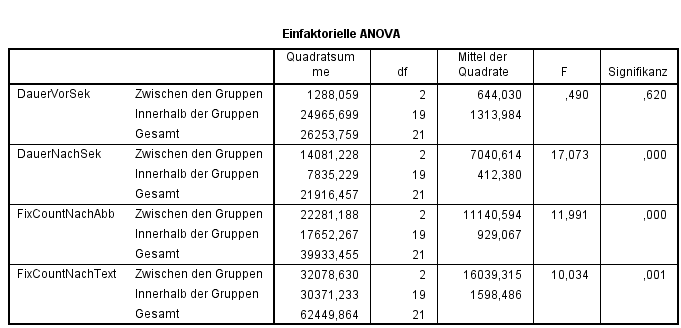
\includegraphics[width=15cm]{./Ressourcen/Gruppenunterscheidung.png}
\caption{Gruppenvarianz, Lorenz Müller}
\end{figure}

Wenn man sich der zweiten Vorschungsfrage widment. Kommt man zu folgenden Ergebnissen:
Alle Studenten erziehlten im Schnitt 6,03 Punkte. 
Die jeweiligen Gruppen erziehlten insgesamt über alle Aufgaben im Durchschnitt folgende Punkte:

\begin{table}[!h]
\hspace{-5pt}
\begin{tabularx}{\textwidth + 5pt}{| @{\hspace{3pt}} M || @{\hspace{3pt}} M  | @{\hspace{3pt}} M | @{\hspace{3pt}} M |}
\hline
\textbf{ } & \textbf{Typ Unsicher} & \textbf{Typ Problemlöser} & \textbf{Typ Textuell}\\
\hline
\hline
Punkte        & 6,17 & 5,5 & 6,3\\
\hline
\end{tabularx}
\caption{Mittelwert der Punkte}
\end{table}


Bei der Untesuchung nach signifikanten Unterschieden wurde
die Varianzanalyse über die Gesamtpunktzahl angestellt, welche folgende Ergebnisse hervorbringt:

\begin{figure}[!ht]
\noindent\hspace{0.5mm}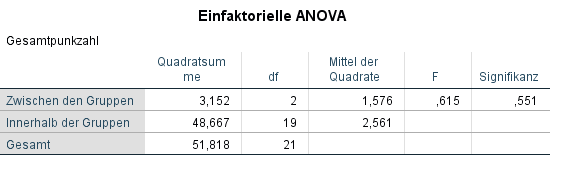
\includegraphics[width=15cm]{./Ressourcen/Punktevarianz.png}
\caption{Punktevarianz, Lorenz Müller}
\end{figure}

Wendet man sich nun der dritten Forschungsfrage, des Einflusses der gewählten Bilder zu, ergibt sich.
Betrachtet man die Beantwortung der einzelnen Aufgaben von allen Probanden.

\begin{table}[!h]
\hspace{-5pt}
\begin{tabularx}{\textwidth + 5pt}{| @{\hspace{3pt}} M || @{\hspace{3pt}} M  | @{\hspace{3pt}} M | @{\hspace{3pt}} M |}
\hline
\textbf{Aufgabe} & \textbf{Radfahrerin 1} & \textbf{Radfahrerin 2} & \textbf{Rennfahrer} \\
\hline
\hline
Prozent richtig beantwortet       & 97,5 & 17,9 & 76,9 \\
\hline
\end{tabularx}
\caption{Mittelwert der Punkte}
\end{table}

\begin{table}[!h]
\hspace{-5pt}
\begin{tabularx}{\textwidth + 5pt}{| @{\hspace{3pt}} M | @{\hspace{3pt}} M  | @{\hspace{3pt}} M | @{\hspace{3pt}} M |}
\hline
\textbf{Zufall} & \textbf{Berg 1} & \textbf{Berg 2} & \textbf{Autofahren}\\
\hline
\hline
    51,3 & 76,9 & 74,3 &  94,9\\
\hline
\end{tabularx}
\caption{Mittelwert der Punkte}
\end{table}

Im Schnitt wurden somit die jeweiligen Bildtypen zu folgenden Prozentwerten richtig beantwortet. 

\begin{table}[!h]
\hspace{-5pt}
\begin{tabularx}{\textwidth + 5pt}{| @{\hspace{3pt}} M || @{\hspace{3pt}} M  | @{\hspace{3pt}} M | @{\hspace{3pt}} M |}
\hline
\textbf{Aufgabentyp} & \textbf{dekorativ} & \textbf{essenziell} \\
\hline
\hline
Prozent richtig beantwortet       & 66,7 & 74,3 \\
\hline
\end{tabularx}
\caption{Mittelwert der Punkte}
\end{table}

Bei der Untersuchung nach signifikanten Unterschieden ergibt sich bei der Varianzanalyse:


Wiedmet man sich nun der vierten Vorschungsfrage:
Werden bei der Auswetung der einzelnen Gruppen auf die Fragen Ergebnisse fett markiert, welche sich um mehr als 20 Prozent vom Wert der Allgemeinheit unterscheiden:

\begin{table}[!h]
\hspace{-5pt}
\begin{tabularx}{\textwidth + 5pt}{| @{\hspace{3pt}} M || @{\hspace{3pt}} M  | @{\hspace{3pt}} M | @{\hspace{3pt}} M |}
\hline
\textbf{Aufgabe} & \textbf{Radfahrerin 1} & \textbf{Radfahrerin 2} & \textbf{Rennfahrer} \\
\hline
\hline
Prozent richtig beantwortet       & 100 & 10 & 90 \\
\hline
\end{tabularx}
\caption{Typ Problemlöser bei den unteschiedlichen Aufgabenstellungen 1}
\end{table}


\begin{table}[!h]
\hspace{-5pt}
\begin{tabularx}{\textwidth + 5pt}{| @{\hspace{3pt}} M | @{\hspace{3pt}} M  | @{\hspace{3pt}} M | @{\hspace{3pt}} M |}
\hline
\textbf{Zufall} & \textbf{Berg 1} & \textbf{Berg 2} & \textbf{Autofahren}\\
\hline
\hline
    40 & 60 & 70 &  \textbf{50}\\
\hline
\end{tabularx}
\caption{Typ Problemlöser bei den unteschiedlichen Aufgabenstellungen 2}
\end{table}

\begin{table}[!h]
\hspace{-5pt}
\begin{tabularx}{\textwidth + 5pt}{| @{\hspace{3pt}} M || @{\hspace{3pt}} M  | @{\hspace{3pt}} M | @{\hspace{3pt}} M |}
\hline
\textbf{Aufgabe} & \textbf{Radfahrerin 1} & \textbf{Radfahrerin 2} & \textbf{Rennfahrer} \\
\hline
\hline
Prozent richtig beantwortet       & 83 & 17 & 67 \\
\hline
\end{tabularx}
\caption{Typ Unsicher bei den unteschiedlichen Aufgabenstellungen 1}
\end{table}

\begin{table}[!h]
\hspace{-5pt}
\begin{tabularx}{\textwidth + 5pt}{| @{\hspace{3pt}} M | @{\hspace{3pt}} M  | @{\hspace{3pt}} M | @{\hspace{3pt}} M |}
\hline
\textbf{Zufall} & \textbf{Berg 1} & \textbf{Berg 2} & \textbf{Autofahren}\\
\hline
\hline
    \textbf{83} & 83 & 67 &  100\\
\hline
\end{tabularx}
\caption{Typ Unsicher bei den unteschiedlichen Aufgabenstellungen 2}
\end{table}

\begin{table}[!h]
\hspace{-5pt}
\begin{tabularx}{\textwidth + 5pt}{| @{\hspace{3pt}} M || @{\hspace{3pt}} M  | @{\hspace{3pt}} M | @{\hspace{3pt}} M |}
\hline
\textbf{Aufgabe} & \textbf{Radfahrerin 1} & \textbf{Radfahrerin 2} & \textbf{Rennfahrer} \\
\hline
\hline
Prozent richtig beantwortet       & 100 & 17 & \textbf{100} \\
\hline
\end{tabularx}
\caption{Typ Textuell bei den unteschiedlichen Aufgabenstellungen 1}
\end{table}


\begin{table}[!h]
\hspace{-5pt}
\begin{tabularx}{\textwidth + 5pt}{| @{\hspace{3pt}} M | @{\hspace{3pt}} M  | @{\hspace{3pt}} M | @{\hspace{3pt}} M |}
\hline
\textbf{Zufall} & \textbf{Berg 1} & \textbf{Berg 2} & \textbf{Autofahren}\\
\hline
\hline
    67 & 67 & 67 &  83\\
\hline
\end{tabularx}
\caption{Typ Textuell bei den unteschiedlichen Aufgabenstellungen 2}
\end{table}

Somit sind folgende Ergebnisse Auffällig. Wobei mit Hilfe der Varianzanalyse untersuch wurde, ob diese sich signifikant von der Allgemeinheit unterscheiden. 

\begin{itemize}
    \item Autofahrt wurde von dem Typ Problemlöser mit nur 50 Prozent richtig gelöst. (Allgemeinheit 94,9 Prozent)
    \item Zufall wurde von dem Typ Unsicher mit 83,3 Prozent richtig gelöst. (Allgemeinheit 0,513)
    \item Rennfahrer wurde von Typ Textuell von allen Probanden richtig gelöst. (Allgemeinheit 0,769)
\end{itemize}

Betrachtet man noch abschliesend, wie sich die unterschiedlichen Lerntypen mit den Bildtypen verhalten haben, so ergibt sich folgende Tabelle.

\begin{table}[!h]
\hspace{-5pt}
\begin{tabularx}{\textwidth + 5pt}{| @{\hspace{3pt}} M | @{\hspace{3pt}} M  | @{\hspace{3pt}} M | @{\hspace{3pt}} M |}
\hline
\textbf{Lerntyp} & \textbf{Unsicher} & \textbf{Problemlöser} & \textbf{Textuell}\\
\hline
\hline
    dekorativ & 62,5 & 60 &  62,5\\
\hline
    essenziell & 83,3 & 60,0 &  83,3\\
\hline
\end{tabularx}
\caption{Typ Textuell bei den unteschiedlichen Aufgabenstellungen 2}
\end{table}

Mit der Varianzanalyse: 

\begin{figure}[!ht]
\noindent\hspace{0.5mm}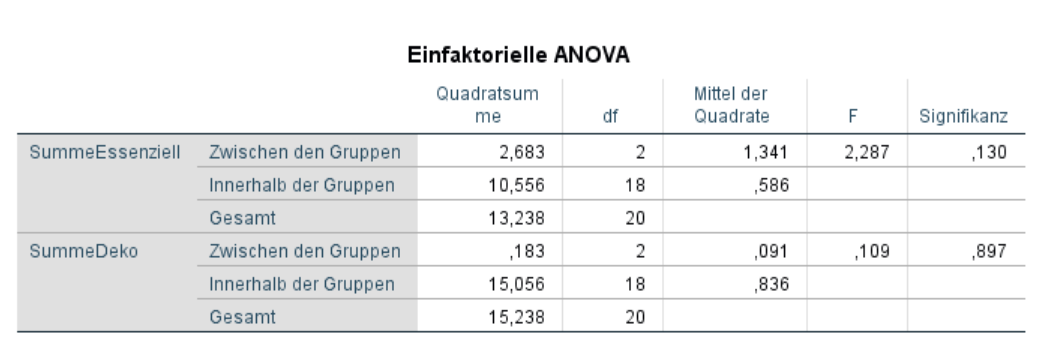
\includegraphics[width=15cm]{./Ressourcen/DekoEssGruppen.png}
\caption{Punktevarianz, Lorenz Müller}
\end{figure}



\chapter{Diskussion}

Wie man aus der Graphik der Gruppenvarianz entnehmen kann unterscheiden sich die Gruppen untereinger in den Merkmalen: Fixationen auf den Text und das Bild jeweils nach dem ersten Durchgang und in der Dauer des zweiten Durchgangs. In der Dauer des ersten Durchgangs ist kein signifikanter Unterschied zwischen den Gruppen festzustellen ($\alpha$ = 0,620 F = 0,490). Dieses Ergebniss Stimmt mit der Theorie überein, dass erstmal der Text von den Probanden linear gelesen wird und erst danach sich die Unterschiede aufzeigen. In der Anzahl der Fixationen auf den Text sowie das Bild dem ersten Durchgang ist ein signifikanter Unterschied festzustellen ($\alpha$ = 0,000 F = 11,991 für das Bild und $\alpha$ = 0,001 F = 10,034 für den Text). Ebenso ist in der Dauer nach dem ersten Durchgang ein Signifikanter Unterschied zu erkennen ($\alpha$ = 0,000 F = 17,073). Also ist die Forschungsfrage (1) mit ja, man kann die Probanden in Gruppen unterscheiden, zu beantworten.

Verwunderlich ist bei der Auswertung der Mittelwerte der Punkte (Forschungsfrage 2), dass die Problemlöser mit 5,5 Punkten im Schnitt am schlechtesten unter den Gruppen abgeschlossen haben. Dieses Ergebniss ist dahingehend verwunderlich, da in der Lerntypeinteilung von Gangé die Problemlöser, welche sich viel mit den unterschiedlichen Darstellungsformen auseinander setzen, hierachisch über den Textuellen, welche sich aus den Grundformen des Lernes nach Gané zusammen setzen sollten. Auf der anderen Seite hat Zech seine Lerntypeinteilung nicht mehr hierarchisch gemacht, was die Ergebnisse weniger verwunderlich erscheinen lässt. Typ Textuell hat in dieser Auswertung mit 6,3 Punkten im Mittel am besten besten Abgeschlossen und er Typ Problemlöser liegt mit 6,17 Punkten im Mittelfeld. Die Punktevarianzabbildung zeigt aber auch, dass die Unterschiede bei den Punkten der einzelnen Gruppen nicht Signifikant sind ($\alpha$ = 0,551 F = 0,615). 

Der folgende Ausdurck von Hyrskykari, Ovaska, Majaranta, Räihä und Lehtinen (2008) erklärt anschaulich was wie leicht es ist Fehlbeurteilungen bei der Untersuchung von Eyetrackingdaten anzustellen:

``Eine markante Zone auf einer Heatmap wird oft als eine interressante Zone interpretiert. Es hat die Aufmerksamkeit des Benutzers auf sich gezogen und deswegen wird angenommen, dass die Zone für den Benutzer jetzt verständlich ist. Dennoch kann aber auch das Gegenteil der Fall sein: Die Zone hat die Aufmerksamkeit des Benutzers angeregt, weil sie verwirrend und problematisch ist und der Benutzer die dargestellte Information nicht(fett) verstanden hat''. (%\cite)

Ebenso haben Similarly, Ballard, Hayhoe und Sullivan (2003) in ihrer Studie gezeigt, dass in manchen Situationen Benutzer direkt auf ein relevantes und wichtiges Objekt schauen und dennoch keine Gedächtnisspur (Wissensgewinn) regestrierbar ist. 

Daraus lässt sich schleißen, dass es nicht so einfach ist die Verhaltensmuster (in unserer Studie Blichbewegungen) der Probanden direkt in ihre kognitiven Prozesse zu übersetzen. Somit ist es leicht sich von den Eyetrackingdaten blenden zu lassen und diese falsch zu interpretieren. In dieser Studie könnten die Probanden aus der Gruppe Problemlöser lediglich viele Fixationen auf den Bildern haben weil sie diese nicht ganz verstanden haben. 

Ebenso ist die Gruppengröße von 6 Probanden in Gruppe Unsicher, 10 Probanden in Gruppe Problemlöser und 6 Probanden in Gruppe Textuell deutlich zu klein um signifikante Ergebnisse zu erzeugen. Man könnte auch sagen diese Gruppengröße hat zu wenig Statistische Aussagekraft um eindeutige Aussagen zu treffen. 

Wenn man sich der dritten Forschungsfrage widmet: In wie fern die Bilder einen Einfluss auf das Ergebniss der Probanden hat. Stellt man schon in den ersten beiden Aufgaben einen Wiederspruch fest: Radfahrerin 1 und Radfahrerin 2 verwenden beide ein dekoratives Bild und ihre Beantwortung fällt im ersten Aufgabenteil sehr gut mit 97,5 Prozent aus und im zweiten Teil, bei dem das selbe dekorative Bild verwendet wurde sehr schlecht mit 17,9 Prozent aus. Hierbei ist durch den Unterschied in der Beantwortung sehr schnell feststellbar, das sich das Niveau der Aufgabenstellung deutlich von dem ersten zu dem zweiten Aufgabenteil unterscheiden muss.

Die beiden Bergaufgaben wurden zu 76,9 und zu 74,3 Prozent richtig bearbeitet, obwohl das beigelegte Bild ebenso nur dekorativ ist. In restlichen Fällen war die verwendete Graphik jeweils essenziell und wurden mit Autofahren 94,9 Prozent, Zufall 51,3 Prozent und Rennfahrer 76,9 Prozent richtig beantwortet. Hierbei wird der Aufgabenteil Zufall auffällig, da er am schlechtesten von den Aufgabenstellungen mit essenziellen Graphiken bewertet wurde. 

Im Durchschnitt über alle Probanden wurden die Aufgaben mit dekorations Bildern zu 66,6 Prozent richtig beantwortet und die Aufgabe mit essenziellen Bildern zu 74,4 Prozent. Dies ist zwar kein signifikanter Untersied, zeigt aber eine Tendenz von dem  Effekt, aus der Studie von Matthias Böckmann und Stanislaw Schukajlow (2018). Mögliche Ursachen wieso der Effekt nicht so groß ist wie erwartet sind: Zum einen wie bereits im ersten Teil geschildert ist der Schwierigkeitsgrad der einzelnen Aufgaben sehr unterschiedlich. Zum anderen ist es ein unterschied, ob man aus einer Graphik lediglich Werte ablesen muss, wie es in Aufgabe Autofahren der Fall ist, oder die Werte stochastisch Auszuwerten, wie es in der Aufgabe Zufall der Fall ist. 

Bei der letzten Forschungsfrage (4) wird gefragt ob bestimmte Aufgabentypen für einzelne Probandengruppen positive oder auch negative Auwirkungen haben. Wie wir in dem Ergebnissteil gesehen haben, werden hierbei drei Fälle einer weiteren Betrachtung unterzogen und versucht eine Erklärung hierfür abzugeben. 

Beginnend mit der schlechten Bearbeitung der Problemlöser, bei der Aufgabe Autofahrt.  Bei dieser Aufgabenstellung war lediglich eine eine Graphik abgebildert, der die Geschwindlichkein mit der Zeit der Autofahrerin in Relation setzt. Gefragt war, ob der linke und höhere Teil (also mehr Geschwindlichkeit)  des Graphen eine größere Strecke darstellt, wie der gleichbeite (also gleiche Zeitdauer) rechte Teil des Graphen.  Hierbei bedeutet der also der der niedrigere Teil (rechts) eine kürzere zurückgelegte Strecke, da   (Weg) x = (Geschwindlichkeit)  v mal t (Zeit) gilt. In der Einstiegsfolie, nach der die Gruppen eingeteilt wurden, war jeweils in den Graphiken, welche sie viel betachtet haben, ganz Eindeutig zu sehen, was mit ihnen gemeint ist. In der Graphik dieser Aufgabe, kann man die gleichbreiten (Zeit) Graphen auch als gleich Weit aus der des zurückgelegten Weges missverstehen.

Im zweiten Fall wurde Zufall von dem Typ Unsicher besonders gut gelöst. In dem Aufgabenteil Zufall sind zwei Graphiken sehen, welche beide ausgewertet und verknüpft werden müssen um die Aufgabenstellung richtig zu beantworten. Der Typ Unsicher hat sich ausgezeichnet indem er auf ersten Folie eine besonders lange zweite Runde mit vielen Fixationen auf Bild und Text gezeigt hat. Diese Dauer kann auch als Gewissenhaft einstuft werden, was ihm in der Aufgabe Zufall zum Vorteil wird, da die beiden Graphiken zuerst abgezählt und dann verküpft werden müssen bevor die Aufgabe beantwortet werden kann. 

Im letzten Teil wurde der Aufgabentyp Rennfahrer von der Gruppe Textuell am besten gelöst. Die Aufgabenstellung war: aus einem gegebenen Graph, welcher die Geschwindlichkeit und die Steckenentfernung in Relation gesetzt hat, den Abstand bis zur längsten geraden Strecke anzugeben. Hierbei konnte dieser Wert einfach aus dem Graphen abgelesen werden, da dieser Wert am Anfang des längsten Teiles ohne Kurve, also Geschwindlichkeits verlust, liegt. Die Gruppe Textuell hat sich auf der ersten Folie dadurch auszezeichnet, dass sie viele Fixationen auf den Text hat. Da der Abstraktionsgrad der Aufgabe Zufall nicht besoders hoch ist, kann durch gewissenhaftest Lesen der Aufgabestellung (des Textes) und einfaches Ablesen des Graphen die Aufgabe erfolgsversprechend gelöst werden. 

Abschließend wenden wir uns noch dem Ergebniss aus der Tabelle XY zu, welche die verschiedenen Lerntypen mit den Bildtypen in Relation setzt. Hierbei fällt auf, das die Unterschiede unter die Gruppen sehr gering sind, mit der Außnahme, dass der Typ Problemlöser schlechter mit den essenziellen Bildtypen umgehen konnte. Dieses Ergebniss steht im Einklang mit dem der Vermutung aus der Disskusion aus Forschungsfrage 1, welche besagt, dass die Problemlöser nicht viele Fixationen auf den Bildern hatten, weil sie sie Verstanden haben, sondern weil es ihnen schwergefallen ist mit ihnen um zu gehen. Auf den Selben Schluss kann man auch bei der Tabelle kommen, das der Typ Problemlöser nicht sehr gut mit den Graphiken arbeiten kann und deswengen essenzielle Bilder schlechter bearbeitet, als die beiden anderen Lerntypen. 


\chapter{Ausblick}
Die Studie zeigt uns, dass sich Lernende in Gruppen anhand von ihren Blickbewegungen in einem gewissen Maße einteilen lassen. Diese Einteilung lässt aber keine direkten Schlüsse auf die mathematische Kompetenz der Probanden zu.  Im Bereich der Verwendung von unterschiedlichen Darstellungsformen, konnten positive Auswirkungen von essenziellen Bildtypen gezeigt werden. Bei der Untersuchung der Lerntypen auf die dargestellen Bildtypen konnte kein besonderer Unterschied gezeigt werden. Aus diesen Ergebnissen sollten sich Lehrkräfte immer bewusst sein, welche Unterstützung sie bei einer Aufgabe geben Möchten. Ebenso ist es gut möglich die SuS selbst zu einer solchen Graphik kommen zu lassen, beispielsweiße mit einer Skitze oder einem Graphen. In einem weiteren Aufgabenteil konnen sie dann ihr selbstkreiertes Bild verwenden, um einer Anschauung zu erhalten. Aufgabentypen wie gerade beschrieben schaffen eine Anschauliche Brücke zwischen der Modelierung eines Problems bis hin zu der Lösung dieses Problems.


Folgende Studien können diese Daten als Grundlage verwenden um sich neue Vorschungsfragen zu überlegen und hierbei Beispielsweise andere Unterteilungen verwenden. Ebenso wäre es Inerresant die gegebene Studie mit einer deutlich größeren Anzahl an Probanden durchzuführen, um die Statistische Aussagekraft der Studie zu verbessern, da in vorliegender Studie lediglich die Gruppen aus 6-10 Probanden bestanden hat.


